\documentclass[12pt]{article}

\usepackage[english]{babel}
\usepackage[utf8]{inputenc}
\usepackage{sansmathfonts}
\usepackage[T1]{fontenc}
\renewcommand*\familydefault{\sfdefault} %% Only if the base font of the document is to be sans serif
\usepackage{multicol,lipsum}
\usepackage{amsmath,cancel}
\usepackage{amssymb,amsthm,dsfont,mathrsfs}
\usepackage[colorinlistoftodos]{todonotes}
\usepackage{geometry}
\geometry{
a4paper,
total={170mm,257mm},
left=20mm,
top=15mm,
bottom=22mm,
}
\usepackage{natbib}
\usepackage{soul}
\usepackage{setspace}
\usepackage{hyperref}
\usepackage{xcolor}
\usepackage{graphicx}
\usepackage{tikz}
\usepackage{siunitx}
\graphicspath{ {imagens/} }
\usepackage{fancyhdr}
\pagestyle{fancy}
\renewcommand{\headrulewidth}{0pt}

\color{darkgray}
\newcommand{\T}[1]{\vspace{0.4cm}\textbf{\large#1}}
\newcommand{\TW}[1]{\textbf{\large#1}}

\newcommand{\TM}[1]{\vspace{0.2cm} \textbf{#1}}

\newcommand{\M}[1]{
\vspace{-0.6cm}
\begin{flalign*}
#1&
\end{flalign*}
\vspace{-0.6cm}
}


\definecolor{bluebell}{rgb}{0.25, 0.35, 0.89} 
\definecolor{laranja}{rgb}{0.87, 0.48, 0.25} 
\definecolor{verde}{rgb}{0, 0.54, 0.44} 
\definecolor{babypink}{rgb}{1, 0.42, 0.52} 
\definecolor{rosa}{rgb}{1, 0.72, 0.77} 
\definecolor{cinza}{rgb}{0.3, 0.3, 0.3}  
\definecolor{iris}{rgb}{0.25, 0.35, 0.89}  
\definecolor{babyblue}{rgb}{0.13, 0.59, 0.95}

\setlength\columnsep{30pt}

\setlength{\parindent}{0cm}
\setlength{\fboxrule}{1.3pt}  % <-- Aumenta a espessura

\newcommand{\Formula}[1]{
\begin{center}
\color{iris}
\fcolorbox{rosa}{white}{
\(
\begin{array}{c}
#1
\end{array}
\)
}
\color{cinza}
\end{center}
}

\begin{document}
\pagenumbering{gobble}
\setstretch{1.3}


\includegraphics[width=4cm]{Logo2.png}
\begin{center}
    \textbf{\Huge \textcolor{bluebell}{Função Logarítmica}}
\end{center}

\begin{multicols}{2}

% ── DEFINIÇÃO ──────────────────────────────────────────────────────────────
\TW{Definição}

A função logarítmica de base $a$ é definida por $f(x) = \log_a x$, onde $a > 0$, $a \neq 1$
e $x > 0$.

\Formula{f(x) = \log_a x, \quad a > 0,\; a \neq 1,\; x > 0}

O \textbf{domínio} é $(0, +\infty)$ e a \textbf{imagem} é $\mathbb{R}$.
A restrição $x > 0$ surge da definição de logaritmo: não existe $\log$ de zero ou negativo.
O gráfico sempre cruza o eixo $x$ no ponto $(1, 0)$, pois $\log_a 1 = 0$.

\TM{Exemplos — $f(x) = \log_2 x$:}

$f(1) = 0$ \quad $f(2) = 1$ \quad $f(4) = 2$

$f\!\left(\tfrac{1}{2}\right) = -1$ \quad $f\!\left(\tfrac{1}{4}\right) = -2$

\TM{Exemplos — $f(x) = \log_{10} x$:}

$f(1) = 0$ \quad $f(10) = 1$ \quad $f(100) = 2$

$f(0{,}1) = -1$ \quad $f(0{,}01) = -2$

\fcolorbox{laranja}{white}{\parbox{0.85\linewidth}{
\small As operações e propriedades dos logaritmos (produto, quociente, potência, mudança
de base) estão em \textbf{Logaritmo}. Este assunto foca na perspectiva de função.
}}

% ── GRÁFICO ────────────────────────────────────────────────────────────────
\TW{Gráfico}

\begin{center}
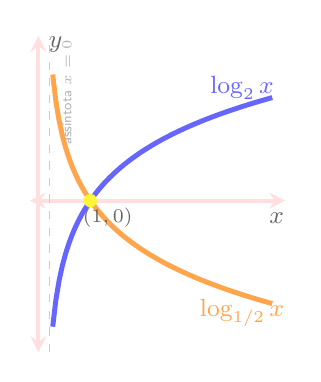
\begin{tikzpicture}[scale=0.55]
\tikzstyle{eixo}=[pink!50!white, line width=1.5pt]
\draw[eixo, stealth-stealth] (-0.2,-3.5) -- (-0.2,3.8);
\draw[eixo, stealth-stealth] (-0.4,0) -- (5.5,0);
\draw[blue!60!white, line width=1.8pt, domain=0.13:5.2, samples=70]
    plot (\x, {ln(\x)/0.6931});
\draw[orange!70!white, line width=1.8pt, domain=0.13:5.2, samples=70]
    plot (\x, {-ln(\x)/0.6931});
\filldraw[yellow!80!white] (1,0) circle (4pt);
\node[black!60!white] at (1.4,-0.4) {\scriptsize$(1,0)$};
\draw[dashed, gray!40!white] (0.05,-3.5) -- (0.05,3.8);
\node[gray!60!white, rotate=90] at (0.45,2.5) {\tiny assíntota $x=0$};
\node[blue!60!white]   at (4.5,2.6) {\small$\log_2 x$};
\node[orange!70!white] at (4.5,-2.6) {\small$\log_{1/2} x$};
\node[black!60!white] at (5.3,-0.4) {\small$x$};
\node[black!60!white] at (0.2,3.6) {\small$y$};
\end{tikzpicture}
\end{center}

$a > 1$: função \textbf{crescente} — assíntota vertical $x = 0$ à esquerda.

$0 < a < 1$: função \textbf{decrescente} — assíntota vertical $x = 0$ à esquerda.

Ambas passam por $(1, 0)$ e têm imagem $\mathbb{R}$.

% ── INVERSA DA EXPONENCIAL ─────────────────────────────────────────────────
\TW{Inversa da Função Exponencial}

$f(x) = \log_a x$ é a \textbf{função inversa} de $g(x) = a^x$:

\Formula{a^{\log_a x} = x \qquad\text{e}\qquad \log_a(a^x) = x}

Geometricamente, os gráficos são \textbf{simétricos em relação à reta $y = x$}.

\TM{Propriedade — inversão de domínio e imagem:}

\vspace{0.2cm}
\begin{center}
\renewcommand{\arraystretch}{1.4}
\begin{tabular}{|l|c|c|}
\hline
Função & Domínio & Imagem \\
\hline
$g(x) = a^x$ & $\mathbb{R}$ & $(0,+\infty)$ \\
\hline
$f(x) = \log_a x$ & $(0,+\infty)$ & $\mathbb{R}$ \\
\hline
\end{tabular}
\end{center}

\TM{Exemplo:}

$(3, 8) \in g(x) = 2^x$ pois $2^3 = 8$.

$(8, 3) \in f(x) = \log_2 x$ pois $\log_2 8 = 3$.

As coordenadas se invertem — reflexão em $y = x$.

% ── ANÁLISE DA FUNÇÃO ──────────────────────────────────────────────────────
\TW{Análise da Função}

Para $f(x) = \log_a x$ com $a > 1$:

\vspace{0.2cm}
\begin{center}
\renewcommand{\arraystretch}{1.4}
\begin{tabular}{|l|l|}
\hline
Domínio & $(0, +\infty)$ \\
\hline
Imagem & $\mathbb{R}$ \\
\hline
Zero & $x = 1$ (para qualquer base) \\
\hline
Sinal & $f < 0$ se $0 < x < 1$; \; $f > 0$ se $x > 1$ \\
\hline
Crescimento & Crescente se $a > 1$; decrescente se $0<a<1$ \\
\hline
\end{tabular}
\end{center}

\TM{Exemplo — inequação logarítmica:}

Para quais $x$ vale $\log_3 x \geq 2$?

Como $a = 3 > 1$ (crescente): $\log_3 x \geq \log_3 9 \;\Rightarrow\; x \geq 9$

$\boxed{x \in [9, +\infty)}$ \hfill {\small(lembrar: $x > 0$)}

\fcolorbox{laranja}{white}{\parbox{0.85\linewidth}{
\small\textbf{Atenção ao sinal da desigualdade:} com $a > 1$ (crescente), o sentido
se mantém. Com $0 < a < 1$ (decrescente), o sentido \textbf{inverte} ao retirar o
logaritmo.
}}

\end{multicols}

\lfoot{\scriptsize © Copyright, Pratique Já}
\cfoot{\large \textcolor{bluebell}{pratiqueja.com}}
\end{document}
